\chapter{ACE-Transfer Integrals} \label{ch:4}

In this chapter, we present an alternative approach for predicting transfer integrals (electronic couplings) of organic molecular dimers using \textsc{ACEpotentials.jl}. Instead of employing standard atomic neighbour representations, we introduce two alternative schemes, namely, \textit{Bead} (\textit{Coarse-Grained}) and \textit{Heavy-atom} representations.

This methodology is motivated by the physical origin of transfer integrals, which are determined by atomic and molecular orbital couplings.
It is therefore reasonable to group the transfer integrals associated with individual atomic orbitals into effective molecular orbitals of a coarse-grained system or to focus specifically on molecular orbitals localised on carbon atoms (e.g., C–H coupling orbitals).

We outline how to build ACE descriptors that are customised to handle various input datasets and  analyse which representations are well suited for different classes of molecular dimers.

Section~\ref{sec:4.1} highlights the significance of transfer integrals in organic semiconductors.
Section~\ref{sec:4.2} provides an analysis of the transfer integral energy surfaces for ring-structured molecular dimers, specifically naphthalene and thiophene dimers. It also covers the construction of ACE descriptors within the \textit{Bead} and \textit{Heavy-atom} frameworks, along with the fitting results and discussions that follow.
In Section~\ref{sec:4.3}, we apply the approach to chain-like molecular dimers (ethylene and 1,1-difluoroethylene), evaluating the predictive capability of the \textit{Bead} and \textit{Heavy-atom} representations within the ACE framework.
Finally, we conclude with a summary of the main findings and outline potential directions for future work in Section~\ref{sec:4.4}.

\section{Transfer Integrals in Organic Semiconductors} \label{sec:4.1}
\begin{figure*}[t]
\centering

\includegraphics[width=0.75\textwidth]{Figure/Chapter 4/MO.jpg}
\caption{\label{fig:4.1} 
Coupling between frontier molecular orbitals (FMOs) of two conjugated organic molecules. The top and bottom FMOs represent the coupling between the lowest unoccupied molecular orbitals (LUMO–LUMO) and the coupling between the highest occupied molecular orbitals (HOMO–HOMO), respectively.
    }
\end{figure*}
%The spatial overlap between FMOs determines the transfer integral $J$ and critically influences charge transport in organic semiconductors.

Organic semiconductors are now essential components for lightweight, flexible electronics. 
Charge carriers in organic materials are frequently localised, unlike in inorganic semiconductors, where charge transport occurs through band-like conduction.

The active layer of the organic semiconductors is typically composed of $\pi$-conjugated molecular systems, in which overlapping $\pi$-orbitals allow for the delocalisation of $\pi$-electrons along the molecular backbone. 
This $\pi$-electron delocalisation facilitates the formation of frontier molecular orbitals, shown in Figure~\ref{fig:4.1}, that are critical for transport processes.

Regarding the discussion in section \ref{sec:2.6}, transport processes can be determined by the electronic coupling between two molecular sites and influence the rate of charge hopping transports, defined as the transfer integrals $J$
\[
J_{ab} = \langle \psi_a | \hat{H} | \psi_b \rangle,
\]
where $\psi_a$ and $\psi_b$ denote the frontier molecular orbitals on the respective molecular sites, and $\hat{H}$ is the electronic Hamiltonian.
Practically, we can parameterise $J_{ab}$ using the relative centre-of-mass displacement $(x_{ab}, y_{ab}, z_{ab})$ and the relative rotational orientations $(\theta_x, \theta_y, \theta_z)$ between two molecules, illustrated in Figure~\ref{fig:4.2}.

\begin{figure*}[t]
\centering

\includegraphics[width=0.65\textwidth]{Figure/Chapter 4/Acceptor.jpg}
\caption{\label{fig:4.2} 
Schematic illustration of charge transport in organic semiconductors. The active layer consists of an intermixed donor/acceptor morphology between anode and cathode electrodes. A zoomed-in view shows the electronic coupling between two $\pi$-conjugated molecules (Mol $a$ and Mol $b$), characterised by their relative centre-of-mass displacement $(x_{ab}, y_{ab}, z_{ab})$ and relative rotational orientations $(\theta_x, \theta_y, \theta_z)$. The transfer integral $J_{ab}$, governing the charge transfer rate between molecules, is a function of these relative coordinates.}
\end{figure*}

In Marcus theory, the transfer integrals can be employed to calculate the charge transfer rate $k$ between two molecular sites, given by
\begin{equation} \label{equ:4.1}
    k = \frac{2\pi}{\hbar} |J|^2 \frac{1}{\sqrt{4\pi\lambda k_B T}} \exp\left( -\frac{(\Delta G + \lambda)^2}{4\lambda k_B T} \right),
\end{equation}

where $\lambda$ is the reorganisation energy, $\Delta G$ is the Gibbs free energy change, $k_B$ is Boltzmann’s constant, and $T$ is the temperature.
The rate depends quadratically on the magnitude of the transfer integral $|J|^2$, implying that precise predictions of $J$ are critical for reliable modelling of charge transport phenomena in organic materials.

However, predicting transfer integrals presents several challenges.
\begin{itemize}
    \item Direct quantum chemical calculations are computationally expensive, particularly for large datasets of molecular dimers \cite{Troisi2011}.
    Accurately computing $J$ typically requires electronic structure methods such as density functional theory (DFT) or fragment orbital approaches, which become prohibitively costly when thousands of molecular configurations must be evaluated, or the molecular assembles contain thousands of atoms.
    \item Transfer integrals are highly sensitive to molecular geometry \cite{Troisi2006}; even small structural perturbations can lead to significant variations in $J$.
    Thermal fluctuations, molecular vibrations, and slight changes in intermolecular orientation can all induce large deviations in the electronic coupling, leading to the difficulty of generalising results across different configurations.
    \item Finally, the development of efficient surrogate models is essential to enable large-scale simulations of charge transport in realistic systems \cite{Fratini2016}.
    Without fast and accurate predictions of $J$, it is impractical to simulate dynamic processes such as charge diffusion over long timescales or in disordered organic materials.
\end{itemize}

Applying a machine learning potential approach, particularly in frameworks based on the atomic cluster expansion (ACE), offers a promising alternative.
By learning the mapping between molecular configurations and transfer integrals, ACE-based models can achieve high predictive accuracy across diverse geometries while significantly reducing computational costs compared to traditional \textit{ab initio} methods.


\section{Fused-ring Dimers} \label{sec:4.2}

This section presents the transfer integral energy surface analysis of ring-structured molecular dimers, with a particular emphasis on naphthalene and thiophene dimers. These fused-ring dimers are rigid and fully parameterised with 6 DoF. Moreover, these two dimer are relatively small, leading to rapid transfer integral calculations. Therefore, it is sensible to begin modelling their transfer integrals as a starting point.

Two alternative frameworks, the \textit{Coarse-Grained} and \textit{Heavy-atom} representations, are employed to construct ACE descriptors. 
Each representation's predictive performance is assessed by fitting the transfer integrals derived from calculations involving quantum chemistry, and the outcomes are then discussed.

We intend to evaluate the ACE methodology's ability to capture the dependence of electronic couplings on molecular configurations by looking at these archetypal Fused-ring systems.

\subsection{Naphthalene} \label{sec:4.2.1}
\subsubsection{Analysis of Transfer Integral Surface}
We begin by investigating the surfaces of the transfer integrals. 
As discussed in Section~\ref{subsec:2.6.4}, many studies predict transfer integrals based on either the square or the absolute value of the transfer integrals, since these quantities correlate linearly with the charge transfer rate.  
However, the surface of the squared transfer integrals $J^2$ is typically discontinuous and highly skewed, containing many small values and a few large peaks, resulting in non-smooth behaviour that poses challenges for machine learning models based on smooth basis sets.
\begin{figure*}[t]\centering
\begin{subfigure}{.33\textwidth}
  \centering
  \includegraphics[width=1\linewidth,height=\textheight,keepaspectratio]{Figure/Chapter 4/1_Naphthalene/naphthalene_J_surface.jpg}
  \caption{}
\end{subfigure}%
\begin{subfigure}{.33\textwidth}
  \centering
  \includegraphics[width=1\linewidth,height=\textheight,keepaspectratio]{Figure/Chapter 4/1_Naphthalene/naphthalene_J^2_surface.jpg}
  \caption{}
\end{subfigure}
\begin{subfigure}{.33\textwidth}
  \centering
  \includegraphics[width=1\linewidth,height=\textheight,keepaspectratio]{Figure/Chapter 4/1_Naphthalene/naphthalene_logJ^2_surface.jpg}
  \caption{}
\end{subfigure}
    \caption{
        \label{fig:4.3}
        (a), (b), and (c) show the surface plots of the transfer integral $J(\theta, \phi)$ of a naphthalene dimer, the squared transfer integral $J^2(\theta, \phi)$, and the logarithm of the squared transfer integral as a function of the rotational angles $\theta$ and $\phi$ for a naphthalene dimer, respectively.
    }
\end{figure*}

Since ACE models are constructed from a set of smooth basis functions, fitting highly non-smooth quantities such as $J^2$ may be particularly sensitive to the choice of basis parameters. 
In such cases, training models directly on the transfer integrals $J$ or on the logarithm of the squared transfer integrals, $\log(J^2)$, can improve predictive capability. 
Both $J$ and $\log(J^2)$ produce distributions that are smoother and more Gaussian-like, which are well suited for regression tasks.

Figures~\ref{fig:4.3} illustrate the three $2d$-surfaces corresponding to the transfer integral of the naphthalene dimer: the transfer integral itself, its squared value, and the logarithm of its squared value. 
These surfaces are parameterised by the orientational angles $\theta \in [0, \pi]$ and $\phi \in [0, 2\pi]$ of molecule $b$ with respect to molecule $a$, as depicted in Figure~\ref{fig:4.2}. 
In other words, molecule $b$ is rotated over the surface of the upper hemisphere around molecule $a$, at a fixed centre-of-mass distance of 12~\AA.
It is evident that the surfaces of the squared transfer integrals (Figure~\ref{fig:4.3}b) and the logarithm of the squared transfer integrals (Figure~\ref{fig:4.3}c) exhibit sharp singularities, whereas the transfer integrals $J$ (Figure~\ref{fig:4.3}a) are smoother by comparison.
This observation suggests that choosing appropriate target quantities, such as $J$ or $\log(J^2)$, is critical for achieving efficient and accurate ACE model fitting.

\subsubsection{Representing Naphthalene Dimers}
\begin{figure*}[t]\centering
  \centering
  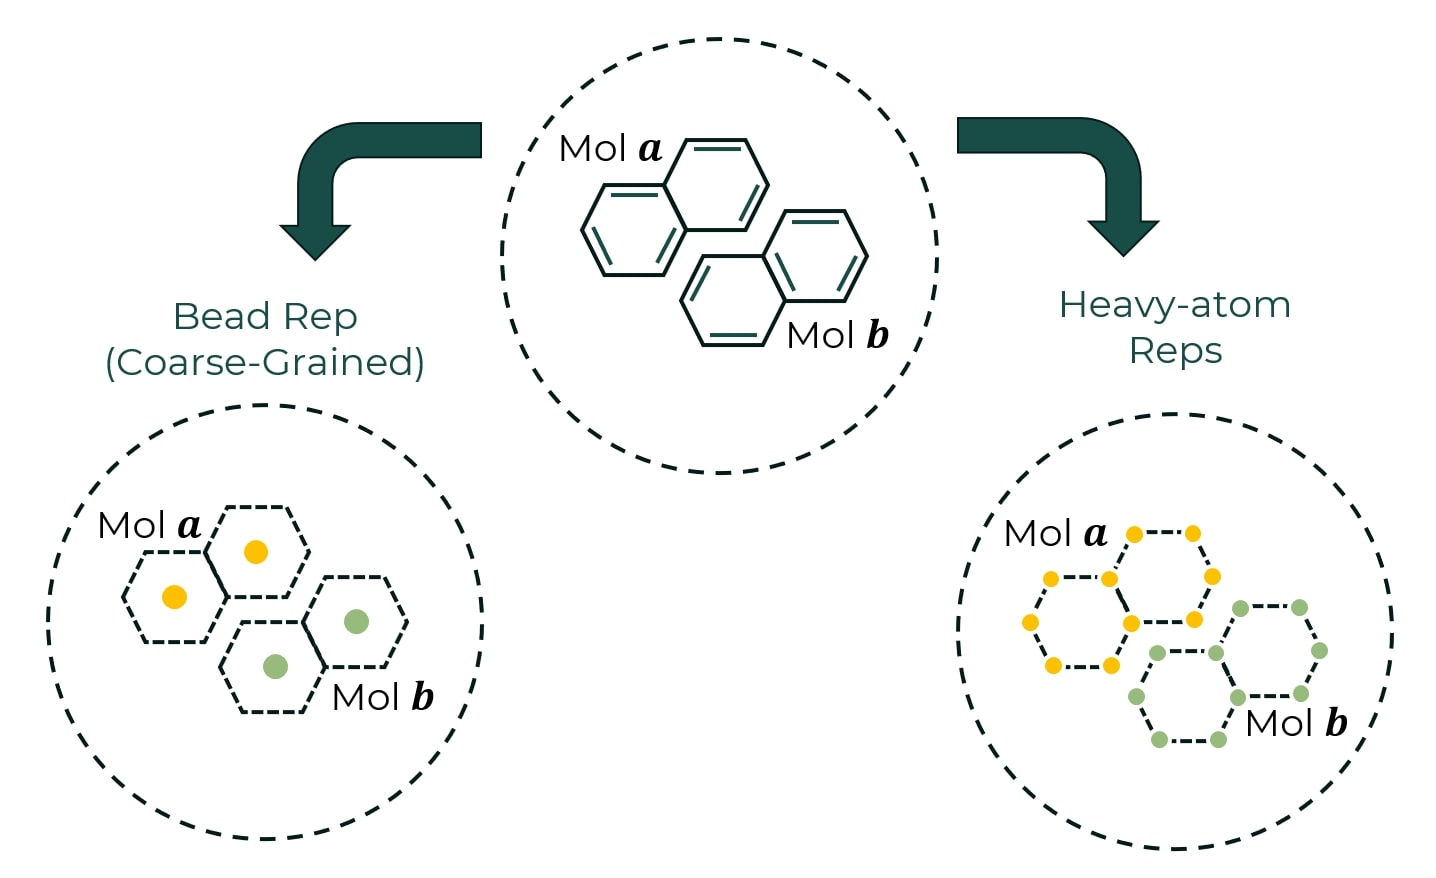
\includegraphics[width=1\linewidth,height=\textheight,keepaspectratio]{Figure/Chapter 4/1_Naphthalene/Representation1.jpg}
    \caption{
        \label{fig:4.4}
        Illustration of two types of molecular representations used for constructing ACE descriptors. The central diagram shows a dimer of Naphthalene (Mol~$a$ and Mol~$b$). The left pathway depicts the \textit{Bead} (\textit{coarse-grained}) representation, in which each aromatic ring is represented by a single Bead. The right pathway illustrates the \textit{Heavy-atom} Representation, where only heavy (Heavy-atom) atoms are included. 
    }
\end{figure*}

Before constructing the ACE descriptors, we introduce an efficient representation of the naphthalene dimer aimed at reducing the dimensionality of the descriptor space while preserving key geometric and electronic features relevant to transfer integral prediction.

One such approach is the \textit{Bead} or \textit{Coarse-Grained Representation}, illustrated on the left pathway of Figure~\ref{fig:4.4}. This method is inspired by the recent work of Wang et al.~\cite{https://doi.org/10.48550/arxiv.2502.04661}, in which ACE models were successfully applied to coarse-grained molecular dynamics. We adapt this idea to model electronic coupling (transfer integrals) by constructing Bead ACE descriptors tailored to dimer interactions.

\begin{figure*}[t]\centering
  \centering
  \includegraphics[width=1\linewidth,height=\textheight,keepaspectratio]{Figure/Chapter 4/1_Naphthalene/RDF_Bead.jpg}
    \caption{
        \label{fig:4.5}
        Analysis of radial distribution functions (RDFs) and radial basis functions (RBFs) used in the ACE descriptor construction for the coarse-grained (Bead) representation. The top panel shows the intra- and intermolecular RDFs as a function of pairwise distance $r$, with a dashed line indicating the fixed centre-of-mass separation (12~\AA). The middle and bottom panels display the corresponding RBFs used to represent intra- and intermolecular environments, respectively. 
    }
\end{figure*}
Since the transfer integral is an intermolecular property, it is important to distinguish between atoms (or Beads) belonging to different molecules. As shown in Figure~\ref{fig:4.4}, we assign distinct element labels to each molecule: the yellow Beads in Mol~$a$ are treated as pseudo-\textbf{C} elements, while the green Beads in Mol~$b$ are labelled as pseudo-\textbf{Si} elements. This labelling enforces a separation of molecular environments and ensures that intra- and intermolecular interactions are treated distinctly within the ACE framework.

The next step is to analyse the intra- and intermolecular radial distribution functions (RDFs), plotted as a function of Bead-pairwise distance in the top panel of Figure~\ref{fig:4.5}.
The yellow histogram represents the intra-molecular RDF, while the red histogram shows the distribution of intermolecular pair distances. 
The dashed vertical line indicates the fixed centre-of-mass separation (12~\AA) used in our dimer configurations.

The analysis of the RDF guides the construction of radial basis functions (RBFs) using the \texttt{acemodel()} function, as illustrated in Figure~\ref{fig:4.6}. A discussion of the relevant hyperparameters is provided in Section~\ref{subsec:3.3.1}. 

\begin{figure*}[t]
  \centering
  \begin{lstlisting}[language=Julia]
model = (*@\textcolor{bEpic}{acemodel}@*)(elements = [(*@\textcolor{rEpic}{:C}@*),(*@\textcolor{rEpic}{:Si}@*),],
        order = 2,                 #3-body order
        totaldegree = 10,
        r0 = 12.0,                
        rcut = 13.6,
        pair_transform = ((*@\textcolor{rEpic}{:agnesi}@*), p = 19, q = 43),
        pair_envelope = ((*@\textcolor{rEpic}{:x}@*), 2, 2),
        Eref = [(*@\textcolor{rEpic}{:C}@*) => 0.0, (*@\textcolor{rEpic}{:Si}@*) => 0.0]
    )
  \end{lstlisting}
  \caption{\label{fig:4.6} Construction of a 3-body order ACE descriptor for a Bead structure using a total degree constraint of 10, an Agnesi radial transform, and a smooth polynomial envelope.}
\end{figure*}
%	@show length(model.basis)
%(*@\textcolor{bEpic}{> length(model.basis)}@*) = 338

Here, we emphasise the role of the envelope function used in constructing the RBFs. The default envelope \texttt{pair\_envelope = (:r, 2, 2)} leads to basis functions extending across both intra- and intermolecular regions (middle panel of Figure~\ref{fig:4.5}).
As shown in the bottom panel, modifying the envelope to \texttt{(:x, 2, 2)} localises the RBFs to the intermolecular range only.
In other words, RBFs are adapted to the relevant intermolecular RDF support ranges, enabling resolution where features are concentrated.
This ensures that the descriptor focuses on features relevant to transfer integrals, which are by nature intermolecular.

An additional hyperparameter, \texttt{Eref}, defines the one-body (atomic reference) energy.
By setting \texttt{Eref = 0} for each Bead type, we enforce the physical constraint that the transfer integral vanishes for isolated molecules or Beads.

\begin{figure*}[t]\centering
  \centering
  \includegraphics[width=1\linewidth,height=\textheight,keepaspectratio]{Figure/Chapter 4/1_Naphthalene/RDF_NH.jpg}
    \caption{
        \label{fig:4.7}
        Analysis of naphthalene dimer RDFs and RBFs used in the ACE descriptor construction for the Heavy-atom representation.
        The upper panel shows the intra- and intermolecular RDFs as a function of pairwise distance , with a dashed line indicating the fixed centre-of-mass separation of 12~\AA.
        The lower panel depicts the corresponding RBFs used to capture only intermolecular environments. 
    }
\end{figure*}
For the \textit{Heavy-atom Representation} shown on the right pathway in Figure~\ref{fig:4.4}, a similar analysis can be performed to construct the radial basis set for the corresponding ACE descriptors. 
In this representation, only heavy atoms (typically carbon) are included, thereby retaining chemically relevant geometric features while reducing the descriptor size.

The radial distribution functions (RDFs) for this representation are shown in the top panel of Figure~\ref{fig:4.7}, plotted as a function of pairwise distances between carbon atoms. 
As in the coarse-grained case, the yellow histogram corresponds to intramolecular RDFs, while the red histogram captures intermolecular distances. The fixed centre-of-mass separation is again marked by a dashed vertical line.

The choice of envelope functions for the radial basis can follow the same design as used in the Bead representation. 
Specifically, by applying an intermolecular envelope (e.g., \texttt{(:x, 2, 2)}), the radial basis functions can be restricted to the intermolecular distance range, thereby focusing the model on the features most relevant for predicting transfer integrals.

\subsubsection{ACEfit!}
\begin{figure*}[t]\centering
\begin{subfigure}{.5\textwidth}
  \centering
  
\includegraphics[width=1\linewidth,height=\textheight,keepaspectratio]{Figure/Chapter 4/1_Naphthalene/fitting_Bead_CSi_od2_td10_p19_q43_rcut136.jpg}
  \caption{}
\end{subfigure}%
\begin{subfigure}{.5\textwidth}
  \centering
  
\includegraphics[width=1\linewidth,height=\textheight,keepaspectratio]{Figure/Chapter 4/1_Naphthalene/fitting_NH_CSi_od2_td10_p19_q43_rcut136.jpg}
  \caption{}
\end{subfigure}
    \caption{
        \label{fig:4.8}
        The plots comparing predicted and reference energies for ACE models trained on 900 structures out of a total of 3,853 dimer configurations. (a) Model trained using the \textit{Bead} representation. (b) Model trained using the \textit{Heavy-atom} representation. Yellow and green markers represent predictions on the full dataset and the training set, respectively.
    }
\end{figure*}
With all descriptors and hyperparameters defined, we now proceed to fit the ACE model to the transfer integral data of the naphthalene dimer. The reference transfer integrals were computed using the \textsc{PyMOO}, ZINDO-based method~\cite{Kirkpatrick2007}, package as implemented by J. M. Frost.

The ACE models constructed using the descriptors in Figure~\ref{fig:4.6} were trained on 900 dimer configurations out of a total of 3,853. The resulting fits using the \textit{Bead} and \textit{Heavy-atom} representations are shown in Figures~\ref{fig:4.8}a and~\ref{fig:4.8}b, respectively. Both models achieve high accuracy in predicting transfer integrals. The Bead-based model yields a root-mean-square error (RMSE) of 12.699~meV/Bead (equivalent to 2.526~meV/atom) and a mean absolute error (MAE) of 8.967~meV/Bead (1.793~meV/atom). In comparison, the Heavy-atom model achieves even lower errors: RMSE = 1.775~meV/atom and MAE = 1.236~meV/atom.

These results are notable in that the predictive errors are of similar magnitude across the two representations, yet the computational cost of the Bead-based model is significantly lower—by approximately a factor of five. The Bead representation uses only four coarse-grained Beads per naphthalene dimer, while the Heavy-atom representation employs twenty carbon atoms per configuration. This efficiency gain results from the reduced number of sites per configuration.

Therefore, the Bead (or coarse-grained) representation may offer an advantage in high-throughput screening scenarios where computational efficiency is critical. On the other hand, when maximal predictive accuracy is required—for example, in detailed mechanistic studies or high-fidelity simulations—the Heavy-atom model provides superior performance.
\begin{figure*}[t]\centering
\begin{subfigure}{.45\textwidth}
  \centering
  \includegraphics[width=1\linewidth,height=\textheight,keepaspectratio]{Figure/Chapter 4/1_Naphthalene/od_error.jpg}
  \caption{}
\end{subfigure}%
\begin{subfigure}{.45\textwidth}
  \centering
  \includegraphics[width=1\linewidth,height=\textheight,keepaspectratio]{Figure/Chapter 4/1_Naphthalene/td_error.jpg}
  \caption{}
\end{subfigure}
    \caption{
        \label{fig:4.9}
        Hyperparameter sensitivity analysis of ACE models fitted to transfer integrals using Bead (yellow) and Heavy-atom representations (green). (a) RMSE (solid) and MAE (dash-dot) as a function of interaction order ($\nu$), which controls the maximum $(\nu+1)$ body order of the ACE descriptor. (b) RMSE and MAE as a function of the total polynomial degree used in the basis.
    }
\end{figure*}

We also provide an analysis of hyperparameter fine-tuning with respect to the \texttt{order} (interaction order) and \texttt{totaldegree} parameters. Figure~\ref{fig:4.9} presents the performance of ACE models fitted to transfer integrals using Bead (yellow lines) and Heavy-atom (green lines) representations. Additional fine-tuning on these two hyperparameters is provided in Appendix~\ref{sec:A.3.1} and \ref{sec:A.3.2}, respectively.

Panel (a) shows the root-mean-square error (RMSE) and mean absolute error (MAE) as a function of the interaction order $\nu$, which determines the maximum $(\nu + 1)$-body correlation captured in the ACE descriptor. As expected, increasing the interaction order improves accuracy for both representations, although with diminishing returns beyond $\nu = 4$.

Panel (b) illustrates the effect of increasing the total polynomial degree. Both representations benefit from increasing \texttt{totaldegree} up to a point of saturation (\texttt{totaldegree} $= 20$), after which performance plateaus or slightly worsens due to overfitting or numerical instability.

We can also see that this fine-tuning analysis supports the earlier discussion for Figure~\ref{fig:4.8}, confirming that the Heavy-atom representation consistently achieves lower errors than the Bead-based model across these two tested hyperparameter settings.

\begin{figure*}[t]\centering
\begin{subfigure}{.5\textwidth}
  \centering
  \includegraphics[width=1\linewidth,height=\textheight,keepaspectratio]{Figure/Chapter 4/2_Thiophene/od_basis.jpg}
  \caption{}
\end{subfigure}%
\begin{subfigure}{.5\textwidth}
  \centering
  \includegraphics[width=1\linewidth,height=\textheight,keepaspectratio]{Figure/Chapter 4/2_Thiophene/td_basis.jpg}
  \caption{}
\end{subfigure}
    \caption{
        \label{fig:4.10}
        Growth of ACE basis size as a function of key hyperparameters for 2- (solid) and 4- (dashdot) chemical species. (a) Basis size also grows rapidly with the interaction order ($\nu$), reflecting the combinatorial increase in many-body terms. (b) Basis size increases exponentially with the total degree of polynomials.
    }
\end{figure*}
However, these improvements in accuracy come with an increased computational cost.
As shown in Figure~\ref{fig:4.10}, the size of the ACE basis set for 2-chemical species grows rapidly with both \texttt{order} and \texttt{totaldegree} values.
Higher values lead to a substantial increase in both memory usage and model training time.
These trends emphasise the compensation between model expressivity and computational efficiency in ACE model construction.

We also further analysed and fine-tunde additional hyperparameters, including cutoff radias \texttt{rcut}, parameters \texttt{p}, and \texttt{q} for controlling the envelop function of RBFs. 
The corresponding ACE fitting results and discussions, provided in Appendix~\ref{sec:A.3}, will justify the suitable range of these hyperparameters for bith Bead and Heavy-atom representation.


In the following sections, we apply the same analysis workflow to predict the transfer integrals of three additional molecular dimers: thiophene, ethylene, and 1,1-difluoroethylene. For these systems, the reference transfer integrals were generated using the \textsc{xtb-dipro} package~\cite{Kohn2023}, rather than \textsc{PyMOO}.
As discussed in Section~\ref{subsec:2.6.3}, \textsc{xtb-dipro} leverages a semi-empirical tight-binding framework, offering significantly lower computational costs compared to conventional density functional theory (DFT) methods. This makes it particularly well-suited for generating large datasets required for ACE model training.

\newpage
\subsection{Thiophene} \label{sec:4.2.2}
\begin{figure*}[t]\centering
\begin{subfigure}{.33\textwidth}
  \centering
  \includegraphics[width=1\linewidth,height=\textheight,keepaspectratio]{Figure/Chapter 4/2_Thiophene/thiophene_J_surface.jpg}
  \caption{}
\end{subfigure}%
\begin{subfigure}{.33\textwidth}
  \centering
  \includegraphics[width=1\linewidth,height=\textheight,keepaspectratio]{Figure/Chapter 4/2_Thiophene/thiophene_J^2_surface.jpg}
  \caption{}
\end{subfigure}
\begin{subfigure}{.33\textwidth}
  \centering
  \includegraphics[width=1\linewidth,height=\textheight,keepaspectratio]{Figure/Chapter 4/2_Thiophene/thiophene_logJ^2_surface.jpg}
  \caption{}
\end{subfigure}
    \caption{
        \label{fig:4.11}
        (a), (b), and (c) show the surface plots of the transfer integral $J(\theta, \phi)$ of a thiophene dimer, the squared transfer integral $J^2(\theta, \phi)$, and the logarithm of the squared transfer integral as a function of the rotational angles $\theta$ and $\phi$ for a naphthalene dimer, respectively.
    }
\end{figure*}
\subsubsection{Analysis of Transfer Integral Surface}
We first examine the energy surfaces of the transfer integrals for the thiophene dimer, as shown in Figure~\ref{fig:4.11}. Panels (a), (b), and (c) illustrate the surfaces of the transfer integral $J$, its squared value $J^2$, and the logarithm of the squared value $\log(J^2)$, respectively.

These surfaces are generated by systematically rotating molecule~$b$ over the upper hemisphere around molecule~$a$, while maintaining a fixed centre-of-mass distance of 6~\AA.
The orientations are parameterised by the angular coordinates $\theta \in [0, \pi]$ and $\phi \in [0, 2\pi]$.

This visualisation helps to determine the most suitable target quantity for ACE model training. Despite some local skewness and discontinuities, the transfer integral surface $J$ appears noticeably smoother than those of $J^2$ and $\log(J^2)$, supporting its selection as a more appropriate target for regression with smooth basis function models such as ACE.

\subsubsection{Representing Thiophene Dimers}

\begin{figure*}[t]\centering
  \centering
  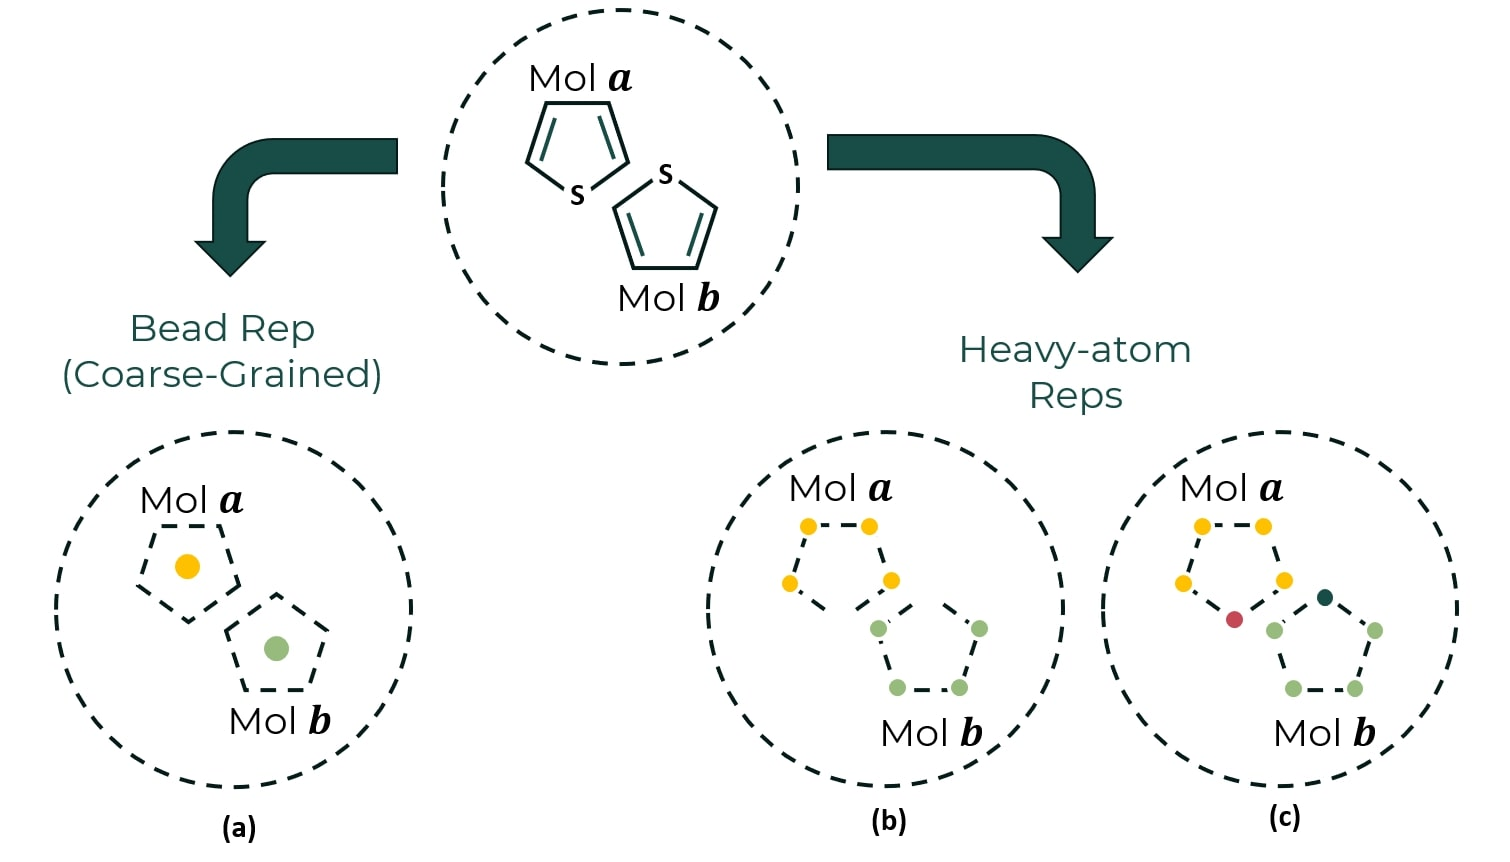
\includegraphics[width=1\linewidth,height=\textheight,keepaspectratio]{Figure/Chapter 4/2_Thiophene/Representation2.jpg}
    \caption{
        \label{fig:4.12}
        Illustration of three types of molecular representations used for constructing ACE descriptors for the thiophene dimer (Mol~$a$ and Mol~$b$). The central diagram shows the full molecular structures. Panel (a) depicts the \textit{Bead} (\textit{coarse-grained}) representation, in which each thiophene ring is represented by a single Bead. Panels (b) and (c) illustrate variations of the \textit{Heavy-atom} representation: (b) includes only carbon atoms, while (c) incorporates both carbon and sulphur atoms as distinct elements. 
    }
\end{figure*}
We now proceed to construct the ACE descriptors for the thiophene dimer, following the molecular representations illustrated in Figure~\ref{fig:4.12}. 

The left pathway (panel a) shows the \textit{Bead} (\textit{coarse-grained}) representation, where each thiophene ring is abstracted as a single Bead. To distinguish the two molecules, the Bead in Mol~$a$ is labelled as a pseudo-\textbf{C} element (yellow), while the Bead in Mol~$b$ is labelled as a pseudo-\textbf{Si} element (green). This labelling enforces molecule-specific environments, allowing the ACE model to distinguish between intra- and intermolecular interactions.

The right pathway (panels b and c) illustrates two variations of the \textit{Heavy-atom} representation. Panel (b) includes only carbon atoms, while panel (c) includes both carbon and sulphur atoms. The sulphur atoms are assigned distinct element labels (e.g., red and dark green) to ensure that atomic species and molecular origin are treated separately. 
\begin{figure*}[t]\centering
  \centering
  \includegraphics[width=1\linewidth,height=\textheight,keepaspectratio]{Figure/Chapter 4/2_Thiophene/RDF_NH.jpg}
    \caption{
        \label{fig:4.13}
        Analysis of thiophene dimer RDFs and RBFs used in the ACE descriptor construction for the Heavy-atom representation.
        The upper panel shows the intra- and intermolecular RDFs as a function of pairwise distance, with a dashed line indicating the fixed centre-of-mass separation of 6~\AA.
        The lower panel depicts the corresponding RBFs used to capture only intermolecular environments. 
    }
\end{figure*}

Again these representations enable a reduction in descriptor dimensionality while preserving essential geometric and electronic features relevant to transfer integral prediction. Moreover, the labelling strategy ensures clear separation of intra- and intermolecular contributions in the ACE basis.

As a next step, we analyse the radial distribution functions (RDFs) for intra- and intermolecular interactions. These are plotted as a function of pairwise distance between the atoms in the thiophene dimer in the top panel of Figure~\ref{fig:4.13}. The yellow histogram corresponds to intra-molecular RDFs, while the red histogram represents intermolecular RDFs. The dashed vertical line indicates the fixed centre-of-mass separation (6~\AA) used in the thiophene dimer dataset.
The bottom panel illustrates the RBFs which can be extracted from the ACE model in the following discussion.

For the construction of the ACE model, we adopt the framework illustrated in Figure~\ref{fig:4.6}, applying it to both the Bead representation (Figure~\ref{fig:4.12}a) and the Heavy-atom representation containing only carbon atoms (Figure~\ref{fig:4.12}b). In each case, the parameters \texttt{r0} and \texttt{rcut} are appropriately adjusted to reflect the relevant intermolecular distance ranges observed in the thiophene dimer dataset.
\begin{figure*}[t]
  \centering
  \begin{lstlisting}[language=Julia]
model = (*@\textcolor{bEpic}{acemodel}@*)(elements = [(*@\textcolor{rEpic}{:C}@*),(*@\textcolor{rEpic}{:Si}@*),(*@\textcolor{rEpic}{:S}@*),(*@\textcolor{rEpic}{:O}@*),],
        ..., # c.f. Figure (*@\ref{fig:4.6}@*)
        Eref = [(*@\textcolor{rEpic}{:C}@*) => 0.0,(*@\textcolor{rEpic}{:Si}@*) => 0.0,(*@\textcolor{rEpic}{:S}@*) => 0.0,(*@\textcolor{rEpic}{:O}@*) => 0.0,]
    )
  \end{lstlisting}
  \caption{\label{fig:4.15} The extension of the construction of the ACE basis to support 4-chemical element structures.}
\end{figure*}

Extending the model to the Heavy-atom representation that includes both carbon and sulphur atoms (Figure~\ref{fig:4.12}c) requires additional species which must be introduced to the ACE descriptor. In particular, sulphur atoms in molecules~$a$ and~$b$ are treated as distinct atomic types. For example, the species may be defined as in the code in Fig.~\ref{fig:4.15}.

\begin{figure*}[t]\centering
\begin{subfigure}{.45\textwidth}
  \centering
  
\includegraphics[width=1\linewidth,height=\textheight,keepaspectratio]{Figure/Chapter 4/2_Thiophene/fitting_NH_CSi_od2_td40_p19_q43_rcut136.jpg}
  \caption{}
\end{subfigure}%
\begin{subfigure}{.45\textwidth}
  \centering
  
\includegraphics[width=1\linewidth,height=\textheight,keepaspectratio]{Figure/Chapter 4/2_Thiophene/fitting_NH_CS_SiO_od2_td40_p19_q43_rcut136.jpg}
  \caption{}
\end{subfigure}
    \caption{
        \label{fig:4.14}
        The plots comparing predicted and reference transfer integrals for ACE models trained on 900 structures out of a total of 4,802 thiophene dimer configurations. (a) Model trained using the \textit{Heavy-atom} representation including only carbon atoms. (b) Model trained using the \textit{Heavy-atom} representation incorporating both carbon and sulphur
        atoms. Yellow and green markers represent predictions on the full dataset and the training set, respectively.
    }
\end{figure*}
In this configuration, a pseudo-oxygen label (\texttt{:O}) is assigned to the sulphur atom in Mol~$b$ to ensure that the ACE model distinguishes between chemically identical atoms residing in different molecular environments. This strategy is consistent with the intermolecular nature of transfer integrals and enables explicit encoding of cross-molecular interactions in the basis construction.

\subsubsection{ACEfit!}
The fitting performance of the ACE models for the thiophene dimer is shown in Figure~\ref{fig:4.14}. Both models were trained on 900 structures out of a total of 4,802 and exhibit strong predictive performance, with root-mean-square errors (RMSEs) of 13~meV/atom and 10~meV/atom for the carbon-only and carbon-sulphur representations, respectively. However, these values are notably higher than those obtained for more structurally symmetric systems such as the naphthalene dimer.

This discrepancy can be attributed to the discontinuous and sharply varying features of the thiophene transfer integral surface \( J(\theta, \phi) \), as shown in Figure~\ref{fig:4.11}a. The thiophene ring system's low symmetry and orientation-dependent $\pi$-orbital interactions account for the surface's sudden sign changes and localised ridges. These discontinuities present a significant challenge to smooth-basis models like ACE, which are inherently better suited to learning smooth, differentiable target functions.

By adding more structural and chemical data to the descriptor space, we can enhance the ACE model.  When compared to the carbon-only model (Figure~\ref{fig:4.14}a), the ACE model with explicit sulphur labelling (Figure~\ref{fig:4.14}b) shows better accuracy, suggesting that the incorporation of chemically distinct atomic species enables the model to more accurately represent complex coupling behaviour and anisotropic interactions.

\begin{figure*}[t]\centering
\begin{subfigure}{.45\textwidth}
  \centering
  \includegraphics[width=1\linewidth,height=\textheight,keepaspectratio]{Figure/Chapter 4/2_Thiophene/od_error.jpg}
  \caption{}
\end{subfigure}%
\begin{subfigure}{.45\textwidth}
  \centering
  \includegraphics[width=1\linewidth,height=\textheight,keepaspectratio]{Figure/Chapter 4/2_Thiophene/td_error.jpg}
  \caption{}
\end{subfigure}
    \caption{
        \label{fig:4.16}
        Hyperparameter sensitivity analysis of ACE models fitted to transfer integrals using Bead (yellow) and Heavy-atom representations (green). (a) RMSE (solid) and MAE (dash-dot) as a function of interaction order ($\nu$), which controls the maximum $(\nu+1)$ body order of the ACE descriptor. (b) RMSE and MAE as a function of the total polynomial degree used in the basis.
    }
\end{figure*}

Moreover, by examining the radial distribution functions (RDFs) of the thiophene dimer dataset in Figure~\ref{fig:4.13}, we observe a sharp peak centred around the fixed centre-of-mass separation at 6~\AA. This pronounced accumulation of intermolecular distances results in a highly non-uniform, non-smooth distribution. This results in the ACE model placing disproportionate resolution at this narrow region of configurational space, limiting its ability to generalise across the full interaction range.

In contrast, the radial basis functions (RBFs), shown in the lower panel, are constructed to smoothly span the entire radial domain between \( r_0 \) and \( r_{\mathrm{cut}} \).  The mismatch between the smooth basis  and the strong localisation of the training data  may lead to inefficient representation of key features and the inaccurate model prediction.
\begin{figure*}[t]\centering
  \centering
  
\includegraphics[width=0.475\linewidth,height=\textheight,keepaspectratio]{Figure/Chapter 4/2_Thiophene/fitting_Bead_CSi_od2_td10_p19_q43_rcut136.jpg}
    \caption{
        \label{fig:4.17}
        Analysis of thiophene dimer RDFs and RBFs used in the ACE descriptor construction for the Heavy-atom representation.
        The upper panel shows the intra- and intermolecular RDFs as a function of pairwise distance, with a dashed line indicating the fixed centre-of-mass separation of 6~\AA.
        The lower panel depicts the corresponding RBFs used to capture only intermolecular environments. 
    }
\end{figure*}

This mismatch effect is consistent with the observed insensitivity of the ACE model to increasing the interaction \texttt{order} and the \texttt{totaldegree} parameter, as presented in Figure~\ref{fig:4.16}. Despite raising model complexity as in Fig.~\ref{fig:4.10}, the resolution gain does not translate to performance improvement, likely because the basis set fails to efficiently capture the dominant, localised interactions in the dataset.

Note that we provide the ACE-fitted transfer integrals for the Bead representation illustrated in Figure~\ref{fig:4.17}.  Regardless of the actual target transfer integral values, the flat horizontal distribution of predictions clustered near zero indicates that the resulting fit is obviously unsuccessful. This unsuccessful prediction likely arises from the poor resolution of the Bead representation for small molecules, where each molecule is represented by a single Bead. This corresponding radial distribution function exhibited as a sharp peak indicating the Mol $b$ Bead at the distance of the centre-of-mass separation.  As a result, the ACE model cannot distinguish among different geometric configurations, leading to non-constant predictions across the dataset.

\section{Chained-like molecular Dimers} \label{sec:4.3}

\begin{figure*}[t]\centering
  \centering
  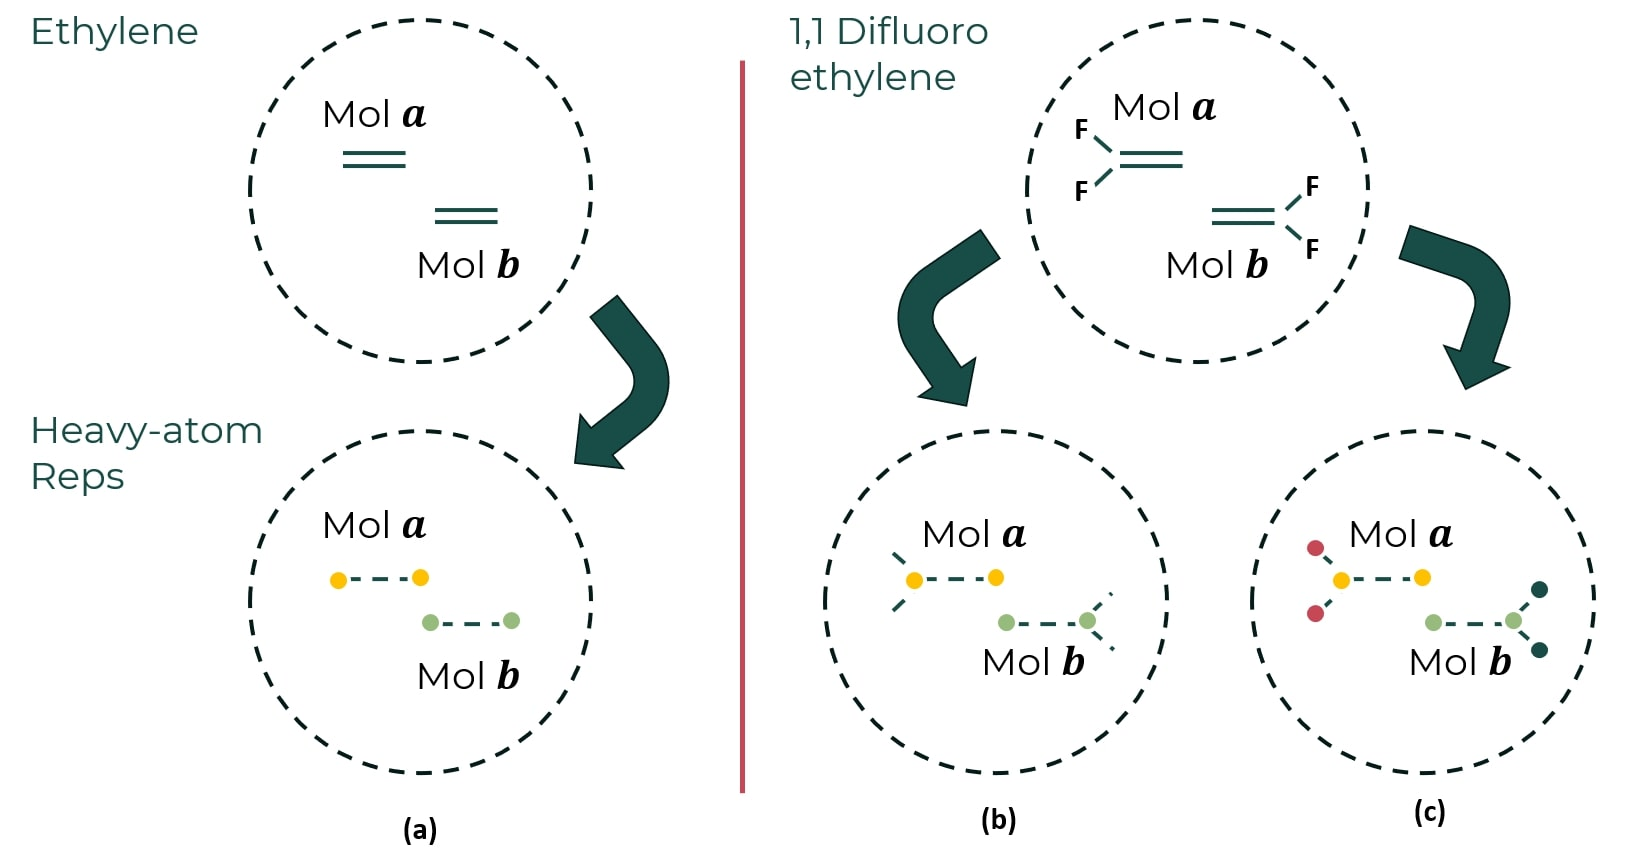
\includegraphics[width=1\linewidth,height=\textheight,keepaspectratio]{Figure/Chapter 4/4_DF_Ethylene/Representation3.jpg}
    \caption{
        \label{fig:4.18}
        Illustration of the \textit{Heavy-atom} representations used for ACE descriptor construction for (left) ethylene and (right) 1,1-difluoroethylene dimers.
        (a) The ethylene dimer is represented using only carbon atoms (yellow and green dots for Mol~$a$ and Mol~$b$, respectively). (b) The 1,1-difluoroethylene dimer includes carbon atoms only, while (c) includes both carbon and fluorine atoms (with red and dark green dots denoting the pseudo-species for fluorine in Mol~$a$ and Mol~$b$, respectively).
        %These representations allow the model to distinguish chemically distinct environments across monomers and are essential for accurately capturing intermolecular electronic couplings.
    }
    
\end{figure*}
In this section, we examine suitable molecular representations for the ethylene and 1,1-difluoroethylene dimers and evaluate the corresponding ACE model predictions of their transfer integrals.

Following the discussion in the previous section, we exclude the \textit{Bead} (coarse-grained) representation from consideration. For small molecules, this representation results in insufficient geometric resolution, which makes it difficult to build effective radial basis sets and leads to poor predictive performance.

We focus on the \textit{Heavy-atom} representation, as illustrated in Figure~\ref{fig:4.18}.  
On the left of the figure, the ethylene dimer is depicted using the standard Heavy-atom representation, incorporating only carbon atoms.  
On the right, we consider two variants for representing the 1,1-difluoroethylene dimer:  
pathway (b) includes only carbon atoms, while pathway (c) incorporates both carbon and fluorine atoms as distinct species.

\begin{figure*}[t]\centering
% First row
\begin{subfigure}{.33\textwidth}
  \centering
  \includegraphics[width=1\linewidth,height=\textheight,keepaspectratio]{Figure/Chapter 4/3_Ethylene/ethylene_J_surface.jpg}
  \caption{}
\end{subfigure}%
\begin{subfigure}{.33\textwidth}
  \centering
  \includegraphics[width=1\linewidth,height=\textheight,keepaspectratio]{Figure/Chapter 4/3_Ethylene/ethylene_J^2_surface.jpg}
  \caption{}
\end{subfigure}%
\begin{subfigure}{.33\textwidth}
  \centering
  \includegraphics[width=1\linewidth,height=\textheight,keepaspectratio]{Figure/Chapter 4/3_Ethylene/ethylene_logJ^2_surface.jpg}
  \caption{}
\end{subfigure}

\vspace{1em} % Space between rows

% Second row
\begin{subfigure}{.33\textwidth}
  \centering
  \includegraphics[width=1\linewidth,height=\textheight,keepaspectratio]{Figure/Chapter 4/4_DF_Ethylene/DFethylene_J_surface.jpg}
  \caption{}
\end{subfigure}%
\begin{subfigure}{.33\textwidth}
  \centering
  \includegraphics[width=1\linewidth,height=\textheight,keepaspectratio]{Figure/Chapter 4/4_DF_Ethylene/DFethylene_J^2_surface.jpg}
  \caption{}
\end{subfigure}%
\begin{subfigure}{.33\textwidth}
  \centering
  \includegraphics[width=1\linewidth,height=\textheight,keepaspectratio]{Figure/Chapter 4/4_DF_Ethylene/DFethylene_logJ^2_surface.jpg}
  \caption{}
\end{subfigure}

\caption{
    \label{fig:4.19}
    Surface plots of an ethylene (upper three plots) and a 1,1 difluoroethylene (lower three plots) dimer transfer integrals as functions of rotational angles $\theta$ and $\phi$. 
    (a) and (d) represent the transfer integral itself. (b) and (e) show the squared transfer integrals, while (c) and (f) depict the surface of their logarithm squared values.
}
\end{figure*}

\subsubsection{Analysis of Transfer Integral Surface and Training Sets }
Figure~\ref{fig:4.19} presents the transfer integral energy surfaces for the ethylene and 1,1-difluoroethylene dimers. Panels (a)–(c) correspond to the ethylene dimer and show the raw transfer integrals \( J \), their squared values \( J^2 \), and the logarithm of the squared values \( \log(J^2) \), respectively. Similarly, panels (d)–(f) display the same quantities for the 1,1-difluoroethylene dimer.
\begin{figure*}[t]\centering
  \centering
  \includegraphics[width=1\linewidth,height=\textheight,keepaspectratio]{Figure/Chapter 4/4_DF_Ethylene/RDF_NH.jpg}
    \caption{
        \label{fig:4.20}
        Radial distribution functions (RDFs) and radial basis functions (RBFs) are used in ACE descriptor construction for ethylene and 1,1-difluoroethylene training sets.
        Top and middle panels show intra- (yellow) and intermolecular (red) RDFs, with a sharp peak at the fixed centre-of-mass separation (dashed line at 6~\AA).
        The bottom panel presents the corresponding RBFs constructed to span the intermolecular distance range. 
    }
\end{figure*}

All surfaces are generated by systematically rotating molecule~$b$ across the upper hemisphere around molecule~$a$, at a fixed centre-of-mass distance of 6~\AA. The orientations are parametrised by spherical angles \( \theta \in [0, \pi] \) and \( \phi \in [0, 2\pi] \). As in the ringed-dimer cases, none of these surfaces exhibit fully smooth or continuous behaviour, which may pose challenges for models based on smooth basis sets such as ACE.

Figure~\ref{fig:4.20} further supports this observation, showing the radial distribution functions (RDFs) of both dimers in the top and middle panels. As with the thiophene dimer, the RDFs exhibit sharp peaks around the centre-of-mass separation, indicating that the local environment is dominated by narrowly distributed intermolecular distances. This leads to poor radial resolution in the feature space and consequently limits the model's representational flexibility.

Note that the apex columns on the surface of the transfer integral exhibit certain irregularities.
As an ethylene dimer possesses a simple structure, its transfer integrals are expected to be uniform and absent of significant peaks over such relative transformation between molecule $a$ and $b$.
These columns certainly are not the result of the contraction of the two ethylenes, as there is no overlap of the intra- and inter-molecular RDFs in the upper panel of Figure~\ref{fig:4.20}.

A possible hypothesis we may propose is that there is an error in the assessment of the eigenvalues associated with ethylene's transfer integrals via \textsc{xtb-dipro} package.
The error could be linked to improper molecular orbital coupling or a phase change of the molecular orbitals due to incorrect molecular orbital projection, during the transformation between molecule $a$ and $b$.
Further investigation is required to assess whether the orbital overlap matrix or Hamiltonian elements are being evaluated consistently across orientations.

\subsubsection{ACEfit!}
Taken together, the highly structured and non-uniform energy landscapes in Figure~\ref{fig:4.19}, along with the narrow RDFs in Figure~\ref{fig:4.20}, explain the limited predictive performance seen in all three fits shown in Figure~\ref{fig:4.21}. These results closely resemble the behaviour previously observed for the Bead-based model applied to the thiophene dimer.

As discussed in the ringed-dimer section, increasing the ACE model complexity—by raising the interaction \texttt{order} and \texttt{totaldegree} parameters—fails to significantly improve predictive performance. This is despite the associated increases in memory usage and computational cost, which grow rapidly with the dimensionality of the basis set.

One possible procedure to address this issue is to enhance sampling across the radial domain. Specifically, generating additional data by varying the centre-of-mass separation between molecules could help populate the sharp peak regions observed in the intermolecular RDFs. This would lead to a more evenly distributed training set and improve the radial resolution of the ACE descriptor.
\begin{figure*}[t]\centering
\begin{subfigure}{.33\textwidth}
  \centering
  
\includegraphics[width=1\linewidth,height=\textheight,keepaspectratio]{Figure/Chapter 4/3_Ethylene/fitting_NH_CSi_od2_td10_p19_q43_rcut136.jpg}
  \caption{}
\end{subfigure}%
\begin{subfigure}{.33\textwidth}
  \centering
  
\includegraphics[width=1\linewidth,height=\textheight,keepaspectratio]{Figure/Chapter 4/4_DF_Ethylene/fitting_NH_CSi_od2_td40_p19_q43_rcut136.jpg}
  \caption{}
\end{subfigure}
\begin{subfigure}{.33\textwidth}
  \centering
  
\includegraphics[width=1\linewidth,height=\textheight,keepaspectratio]{Figure/Chapter 4/4_DF_Ethylene/fitting_NH_CS_SiO_od2_td40_p19_q43_rcut136.jpg}
  \caption{}
\end{subfigure}
    \caption{
        \label{fig:4.21}
        Comparison of ACE model performance for ethylene and 1,1-difluoroethylene dimers using different Heavy-atom representations.
        Panel (a) of the ethylene dimer fitted with a carbon-only representation.
        Panels (b) and (c) of the 1,1-difluoroethylene dimer with carbon-only and both carbon and fluorine representation, respectively, show poor prediction with near-zero flat outputs.
    }
\end{figure*}

One possible procedure to address this issue is to enhance sampling across the radial domain. Specifically, generating additional data by varying the centre-of-mass separation between molecules could help populate the sharp peak regions observed in the intermolecular RDFs. This would lead to a more evenly distributed training set and improve the radial resolution of the ACE descriptor.

Moreover, since the transfer integrals vary smoothly with respect to intermolecular distance—owing to the predominantly Coulombic nature of the interactions—such sampling would yield physically consistent training targets that are more tractable to smooth function approximation. This approach may ultimately enable better generalisation and accuracy in ACE-based models for molecular dimers.

\section{Conclusions and Future Work} \label{sec:4.4}
In this chapter, we introduced an ACE-based method that uses physically motivated representations to predict transfer integrals (electronic couplings) in organic molecular dimers. Two different schemes were presented and assessed for various classes of molecular dimers: the \textit{Bead} (or \textit{Coarse-Grained}) representation and the \textit{Heavy-atom} representation. In order to balance computational efficiency and ACE descriptor resolution, these representations were created to capture important geometric and electronic features related to intermolecular charge transport.

Our findings indicate that the \textit{Heavy-atom} representation consistently outperforms the \textit{Bead} representation in terms of prediction accuracy, particularly for small or chemically heterogeneous systems such as thiophene and 1,1-difluoroethylene. In comparison with larger, more symmetric dimers like naphthalene, both representations produce satisfactory results, even though the Bead-based model offers significant computational advantages due to its reduced dimensionality. However, for smaller dimers such as ethylene, the Bead representation fails entirely, yielding trivial predictions due to insufficient configurational resolution. Across all systems, we observed that the transfer integral surfaces often exhibit discontinuities and sharp features that are challenging to learn using smooth basis sets such as those in ACE. Highly localised radial distribution functions (RDFs) make this problem more severe by reducing the radial basis functions' effective support.

Although increasing the model complexity—by raising the interaction \texttt{order} and \texttt{totaldegree} parameters—leads to a larger basis set, this does not always result in improved predictive performance. The mismatch between the peaked data distributions and the smooth ACE basis leads to inefficiencies and, in some cases, diminishing returns. Consequently, further improvements must come from better alignment between descriptor resolution and the data characteristics.

For future works, there are several promising directions for future work. First, generating training datasets with varied centre-of-mass separations may enhance the radial sampling, thus improving descriptor coverage and reducing interpolation errors. Second, transforming the target quantity—for example, fitting to $\log(J^2)$ instead of $J$ or $J^2$—may improve learning outcomes by producing smoother and more Gaussian-like distributions. Third, integrating ACE descriptors into hybrid architectures such as graph neural networks or message-passing schemes \cite{https://doi.org/10.48550/arxiv.2206.07697, Batatia2025} could offer improved representation of anisotropic and long-range interactions. Additionally, representation learning approaches that optimise atom-type embeddings or construct chemically informed basis functions may improve performance in systems with strong electronic heterogeneity. Finally, applying these ACE-based models to larger-scale simulations of charge transport in organic materials would allow us to assess their utility in realistic device-level scenarios.

To wrap up, this study shows that ACE is a capable and versatile tool for building surrogate models of transfer integrals. The approaches explored here form a solid starting point for further work on machine-learning-based models of charge transport in organic materials. That said, there are still clear challenges—especially for systems that are small, lack symmetry, or involve chemically diverse atoms—where the model struggles to capture all the relevant details.